\begin{frame}
  \frametitle{Encore un peu d'histoire}

  \begin{block}{Newton, Isaac (1642-1727) }
    \begin{columns}[c]
      \begin{column}{.3\textwidth}
        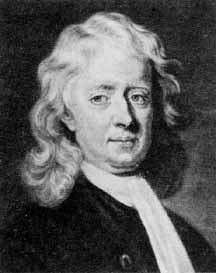
\includegraphics[height=.25\textheight]{figures/jpegs/prudhomme/Newton}
      \end{column}
      \begin{column}{.55\textwidth}
        All in nature reduces to differential equations
      \end{column}
    \end{columns}

  \end{block}

  \begin{block}{Planck, Max (1858-1947)}
    \begin{columns}[c]
      \begin{column}{.3\textwidth}
        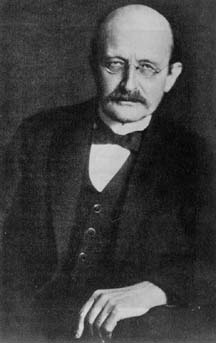
\includegraphics[height=.25\textheight]{figures/jpegs/prudhomme/Planck}
      \end{column}
      \begin{column}{.55\textwidth}
        ...Present day physics, as far as it is theoritically organized,
        is completely governed by a system of space-time differential
        equations.
      \end{column}
    \end{columns}
  \end{block}
 \end{frame}
